% Inspiration: ymca template by Lalit Rai

\documentclass[twoside]{letter}
\usepackage{multicol}
\usepackage{ragged2e}
\usepackage[a4paper]{geometry}
\usepackage{fancyhdr}
\usepackage{amssymb, amsmath, graphicx}
\usepackage{lipsum}
\usepackage[none]{hyphenat}
\usepackage{bookman}
\usepackage{fontenc}

\usepackage[usenames, dvipsnames]{xcolor}
\definecolor{betterblue}{RGB}{0,105,175}
\usepackage[bookmarks, colorlinks, breaklinks, pdftitle={Formal Letter}]{hyperref}
\hypersetup{linkcolor=blue, citecolor=blue, filecolor=black, urlcolor=betterblue}
\usepackage{tikz}

%Margins and Header/Footer
\geometry{a4paper,
  top=2.54cm,
  bottom=2.54cm,
  left=2.54cm,
  right=2.54cm,
  headheight=14.5pt, % the default is too short
  heightrounded, % avoids the need of a flexible baselineskip
} 

\pagestyle{fancy}
\renewcommand{\headrulewidth}{0.4pt}
\renewcommand{\footrulewidth}{0.4pt}
\fancyhf{} % clear all fields
\fancyhead[R]{}
\fancypagestyle{fancy}{%
  \renewcommand{\headrulewidth}{0.4pt}%
  \renewcommand{\footrulewidth}{0.4pt}%
  \fancyhf{}% clear all fields
  \fancyhead[R]{}%
  \fancyfoot{}
}

\renewcommand{\headrulewidth}{0pt}
\renewcommand{\footrulewidth}{0pt}

\setlength\parindent{0pt}
\addtolength{\parskip}{\baselineskip}

%\fancyhead[L]{\bf 00/0000}

\begin{document}

\justifying

\parbox{\linewidth}
{
\begin{flushright}
Rua Cristiano Vianna 104, ap 21\\
\textbf{\textsc{São Paulo}}\\
\mbox{}\\
+55 35 99754-9882\\
\href{mailto:caiolagana@gmail.com}{caiolagana@gmail.com}
\end{flushright}
}

\textbf{\today}

%\parbox{\linewidth}
%{
%\begin{flushleft}
%\emph{Addressee's Job Title}\\
%Department, Organization\\
%\mbox{}\\
%Street/Locality, \textbf{\textsc{City 000 000}}\\
%\end{flushleft}
%}

\vspace{2em}

\begin{center}\textsc{\Large \textbf{Neural Networks in a Nutshell}}\end{center}

Definition. Let $w^l_{jk}$ be a collection of $l$ matrices whose indexes $jk$ are such that the number of columns of the $l$\textsuperscript{th} matrix equals the number of lines of the $(l+1)$\textsuperscript{th} matrix.`'


Definition. The $l$\textsuperscript{th} activation vector, denoted $a^l$, is the (column) vector resulting from the application of the $l$\textsuperscript{th} weight matrix to the $a^{l-1}$ activation vector.
\[
  a^l_j = \sigma \left(\sum_k w^l_{jk}a^{l-1}_k+b^l_j\right)
\]

Definition. A {\bf layer} is the collection of neurons at a given index.

Definition. A {\bf neuron} is 

Example. the following set is a valid collection:
\[
    \begin{pmatrix}
    \cdot & \cdot & \cdot \\
    \cdot & \cdot & \cdot \\
    \cdot & \cdot & \cdot \\
    \cdot & \cdot & \cdot \\
    \cdot & \cdot & \cdot \\
    \end{pmatrix}
    ,
    \begin{pmatrix}
    \cdot & \cdot & \cdot & \cdot & \cdot \\
    \cdot & \cdot & \cdot & \cdot & \cdot \\
    \end{pmatrix}
\]


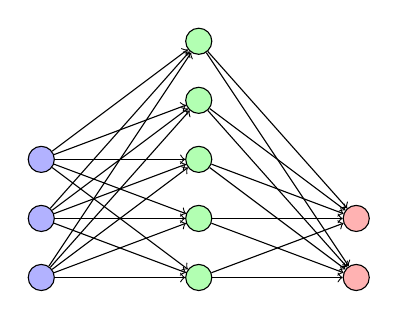
\begin{tikzpicture}
  % Input layer
  \foreach \i in {1,...,3}
      \node[circle, draw=black, fill=blue!30] (input-\i) at (0,\i*0.75) {};

  % Hidden layer
  \foreach \i in {1,...,5}
      \node[circle, draw=black, fill=green!30] (hidden-\i) at (2,\i*0.75) {};

  % Output layer
  \foreach \i in {1,...,2}
      \node[circle, draw=black, fill=red!30] (output-\i) at (4,\i*0.75) {};

  % Connect input layer with hidden layer
  \foreach \i in {1,...,3}
      \foreach \j in {1,...,5}
          \draw[->] (input-\i) -- (hidden-\j);

  % Connect hidden layer with output layer
  \foreach \i in {1,...,5}
      \foreach \j in {1,...,2}
          \draw[->] (hidden-\i) -- (output-\j);

  % Labels
  %\foreach \i in {1,...,3}
  %    \node[left] at (input-\i.west) {Input \i};
  %\foreach \i in {1,...,8}
  %    \node[right] at (hidden-\i.east) {Hidden \i};
  %\foreach \i in {1,...,2}
  %    \node[right] at (output-\i.east) {Output \i};
\end{tikzpicture}



Definition. Let $M_1, M_2, \cdots, M_N$ be a collection of matrices such that the number of columns of the $i$th matrix equals the number of rows of the $(i+1)$th matrix. Let $W_i$ and $B_i$ be ... Each matrix $M$ acts on an input vector $a$ as $M(a)=\sigma(w\cdot a+b)$. Then a Neural Network (NN) is the composition of matrices $T = (M_N \circ M_{N-1} \circ \cdots \circ M_1)$.

Definition. For a given input vector $x$, the prediction vector is defined as $y(x) = T (x)$.


\bigskip

\emph{Cordialmente},

\vfill

    \parbox{\linewidth}
    {
    \begin{flushright}
        \textbf{\emph{Caio Laganá Fernandes}}
    \end{flushright}
    }

\end{document}